%!TEX root = thesis.tex
\chapter{Results for FGK stars}
\label{cha:results}
\epigraph{Don't cry because it's over, smile because it happened.}{Dr. Seuss}

It is time to apply the theory and methodology on some data. In this chapter results from studies
during the thesis will be presented. There is the analysis of three stars which lead to two papers,
HD20010 \citep{Andreasen2016} and Arcturus \& 10 Leo \citep{Andreasen2017b}. Additionally, there was
a analysis of how a cut in EP might affect the final parameters of a star. This will be discussed in
\sref{sec:EPcut}, and last the analysis of a range of synthetic spectra from the PHOENIX spectral
library \citep{Husser2013}, with $T_\mathrm{eff}$ lower than analysed in previous stars with the
methodology described above in \sref{sec:parameters}. However, before diving into the results of the
analysis it is important to describe how the NIR line list were compiled and why and how it was
later refined.


\section{The creation of a NIR line list}
\label{sec:creation_line_list}

As discussed extensively in \cref{cha:theory} and \cref{cha:method}, a atomic line list is needed
for employing the method described here. This line list is made by iron lines in the NIR. This has
already been mentioned in \cref{cha:theory}. Here the process will be explained in greater detail
below for the two versions presented in \citet{Andreasen2016} and \citet{Andreasen2017a},
respectively.


\subsection{First version}

The first version of a NIR iron line list for determining stellar atmospheric parameters of high
resolution and high S/N spectra were presented in \citet{Andreasen2016}. Here all iron transitions
between \SIrange{10000}{25000}{\angstrom}\footnote{That is equivalent to the YJHK bands.} were
downloaded from the VALD database \citep{VALD1,VALD2}. This only includes \ion{Fe}{I} and
\ion{Fe}{II} transitions. In total were \num{50198} \ion{Fe}{I} and \num{28339} \ion{Fe}{II} lines
respectively from the VALD3 database.

The EW of all lines were measured in a solar atlas by \citet{Hinkle1995}. The EWs were measured
using \ARES due to the large amount of lines and to be as consistent as possible in the
measurements. Since \ARES expect a 1D spectrum with equidistant wavelength step, the solar spectrum
were interpolated onto a regular wavelength grid of \SI{0.01}{\angstrom}. This did not change the
appearance, and hence not the EW, of the final spectrum. This wavelength step is equivalent to a
spectral resolution of \num{1500000} at \SI{15000}{\angstrom}.

The EWs are measured by fitting Gaussian profiles to the spectral lines. For a given line, \ARES
output the central wavelength of the line (provided in the line list), the FWHM maximum of the
fitted line, the number of lines fitted for the final result, the depth of the line, the EW of the
line, and the Gaussian coefficients of the line. In the latest version of \ARES, the error of the EW
is also provided \citep{Sousa2015a}. A few lines could not be measured by \ARES and were simply
discarded. It is not completely clear why \ARES had troubles measuring these lines, however, since
the amount was low (less than 1 per thousand) this was not a concern.

More lines were discarded according to the following criteria:

\begin{itemize}
  \item Lines with EW lower than \SI{5}{m\angstrom} as these lines can be problematic to see in
        spectra with lower S/N or spectra with many spectral features.
  \item Lines with EW higher than \SI{200}{m\angstrom} as these lines are too strong to be fitted
        with a Gaussian profile. These lines might also be saturated and do not contain information
        about the abundance (see \fref{fig:cog}).
  \item Lines where the total number of fitted lines are 10 or higher since they show indications of
        severe blending.
  \item If the fitted central wavelength is more than \SI{0.05}{\angstrom} away from the wavelength
        provided by VALD3 to avoid false identification.
\end{itemize}
After this removal the number of \ion{Fe}{I} and \ion{Fe}{II} lines are reduced to \num{6060} and
\num{2735}, respectively.


\subsubsection{Visual removal of lines}

At this point a visual inspection were necessary. All absorption lines from all elements were
downloaded from the VALD3 database in a \SI{3}{\angstrom} window around each of the nearly
\num{9000} iron lines from the previous step. For each small spectral window, all absorption lines
(including the iron line(s)) were plotted on top of the solar spectrum. An iron line were discarded
if another line had the same central wavelength and/or the absorption line were severely blended.
Most of the discarded iron lines had high EP, which are weak compared to the low EP lines.
Therefore, it is fair to assume that many of these iron lines were falsely identified as another
stronger line from another element. After the visual removal the number of \ion{Fe}{I} and
\ion{Fe}{II} lines were reduced to a mere 593 and 22, respectively.

For some of the absorption lines it was not clear which element was the cause. These lines were
marked for further investigation with synthesis as described below.

\subsubsection{Synthetic investigation}

For the lines marked above for further investigation an even broader window were used of
\SI{6}{\angstrom}. Once again, all lines were downloaded from the VALD3 database in these spectral
windows. \MOOG were used with the \emph{synth} driver to create a synthetic spectrum using a solar
atmosphere model with $T_\mathrm{eff}=\SI{5777}{K}$, $\log g=4.438$, $A(\mathrm{Fe})=7.47$, and
$\xi_\mathrm{micro}=\SI{1.00}{km/s}$. The iron abundance (7.47) is from \citet{Gonzalez2000}. The
overall metallicity for the solar atmosphere model is $[\ion{M}/\ion{H}]=0.00$ by definition. This
was done for all spectral windows for three different $A(\mathrm{Fe})=\{-0.2, 0.0, 0.2\}$. Before
creating a synthetic spectrum all elements which are more than singly ionised were removed since
\MOOG does not allow these. An example of this can be seen in \fref{fig:synthetic_investigaton}.

If the three synthetic spectra shows variation at the iron line of interest, then it is assumed that
the iron line is the cause for the absorption line. As a simple test, the iron line was also removed
from the line list used to create the synthetic spectra. If the iron line in the synthetic spectra
disappeared, it was a clear signal that this line can be used in the final iron line list. In some
cases two iron lines had the same or very similar wavelength, and this technique was used to include
the right iron line. In cases where both iron lines causes the absorption line, they were both
discarded since they are blended.

In a few cases two iron lines had the same wavelength and EP but different $\log \mathit{gf}$. If
these both cause an iron line they can be combined into a single line by adding their $\mathit{gf}$
values. After this step, there was 414 \ion{Fe}{I} lines and 12 \ion{Fe}{II} lines, respectively.



\subsubsection{Calibrating $\log \mathit{gf}$}

These lines were collected into a single line list in the format required by MOOG \citep{Sneden1973}
and the line abundance were measured by all lines using the solar atmosphere model described above.
\unfinished{Finish from here...}

\subsection{Second version}





\section{HD20010}
\label{sec:HD20010}

HD 20010 is a star that has been analysed twice with the methodology described here in this thesis.
First time this star was analysed was in \citet{Andreasen2016} when the NIR line list was published.
Later this line list was revised leading to a removal of several lines. This resulted in the second
analysis in \citet{Andreasen2017b}; both described below.

\subsection{First analysis}

To test our new line list we search for a well-studied solar-type star. The spectrum for such a
target needs to be available in the NIR at both high resolution and high S/N. An ideal place to look
for such a star is the CRIRES-POP database (Lebzelter et al. 2012). Here, the best target for
testing is HD 20010, an F8 subgiant star. This star has been part of many surveys and is therefore
well studied. Different parameters from the literature are listed in Table 3. The data available at
CRIRES-POP are in the raw format and pipeline reduced, while three small pieces of the spectra are
fully reduced on the web page 3 . The data is in the standard CRIRES format with each fits file
including four binary tables with the data from the four detectors. In the future, the final reduced
data will be presented by the CRIRES-POP team. In contrast to the pipeline reduced data, this will
be of higher quality, a better wavelength calibration, and telluric correction. We measured the EWs
of the pipeline reduced spectra, and where there was an overlap with the fully reduced spectrum, we
measured both as a consistency check. The measured EWs from the fully reduced spectra were
consistent with the measured EWs from the pipeline reduced spectra. As mentioned above, we use the
Y, J, H, and K-bands which are all available for this star. The spectra come in pieces of 50 Å to
120 Å. These pieces over- lap each other, and we were able to measure the EW for a single line up to
five times. Unfortunately, wavelength calibration is a difficult task for CRIRES owing to the rather
small spectral regions measured on each detector. Each calibration was performed separately for each
detector and required the avail- ability of a sufficient number of calibration lines in the
respective spectral region. This was not always the case and a default linear solution was applied.
A pipeline reduced spectrum shows up as a stretched spectrum if the wavelength calibration is poor
compared to a model spectrum or a solar spectrum, for example. The wavelength calibration does not
have any effect on the signal-to-noise ratio, which is generally high for the spectrum of HD 20010.
The signal-to-noise varies between 200 and 400 for different chunks. The pipeline reduced spectra
for HD 20010 contains tellurics and the wavelength is shifted in radial velocity. All of these
factors make the line identification very difficult, and so we developed a program to properly
identify the lines, which does the following:

\begin{enumerate}
  \item Plotting the observed spectrum
  \item Overplotting a model spectrum. In this particular case the solar spectrum was used since the
        atmospheric parameters are close enough, so the sun was able to serve as a model
  \item Overplotting a telluric spectrum from the TAPAS web page \citep{Bertaux2014}
  \item Overplotting vertical lines at the location of lines in the list
  \item Calculating the cross-correlation function (CCF) for the telluric spectrum with respect to
        the observed spectrum, locating the maximum value by a Gaussian fit, and using this to shift
        the telluric spectrum with the found RV;
  \item Performing the same as step 5, but for the model
  \item Shifting the lines with the same RV as found for the model/solar spectrum.
\end{enumerate}

The final plot shows the shifted spectra, and the CCFs at the sides. An example of the software in
use is shown in Fig. 6. The two RVs are part of the title of the plot. Once the lines were
identified, the EWs were measured with the splot routine in Image Reduction and Analysis Facility
(IRAF). The reason not to choose \ARES for this task was to visually confirm the identification of
the line given the relative poor wavelength calibration. We were able to measure 249 \ion{Fe}{I}
lines and 5 \ion{Fe}{II} lines compared to 344 \ion{Fe}{I} lines and 13 \ion{Fe}{II} lines for the
Sun over the whole NIR spectral region. Whenever we had more than one measurement of a line, the
average was used for the final EW. We derived the stellar parameters using the standard procedure
(see Sect. 2.6) as done for the Sun. Given the relatively low quality of the spectrum of HD 20010
(see below) and be- cause it is not corrected for telluric contamination, we made a cut in EW at
\SI{5}{m\AA{}} in order to remove the lines which are most affected by contamination from either
telluric or other line blends. Additionally, we made a cut in EP at \SI{5.5}{eV} because the
\ion{Fe}{I} and \ion{Fe}{II} lines usually used for stellar parameter determination in the optical
regime are also limited to similar values \citep[see e.g][]{Sousa2008a}. Higher excitation potential
lines are also more likely to be affected by non-LTE effects. When deriving the atmospheric
parameters, we made a $3\sigma$ outlier removal in the abundance iteratively until there were no
more outliers present. Since we could only measure 5 \ion{Fe}{II} lines, for comparison we also
decided to derive parameters using the same method, but we fixed the surface gravity to the
reference value. The resulting atmospheric parameters and iron abundances are presented in Table 4.
The effective temperature, surface gravity, and metallicity agree within the errors with the
literature values. Similar parameters are obtained by fixing log g to the average literature value
or by leaving it free.

The errors on the atmospheric parameters for HD 20010 are much higher than what is achievable with
other measurements in the literature, as presented above in Table 3. In order to explain these
errors, we calculated the abundances for all lines which have at least two measurements of the EW.
We then calculated the abundances for the highest measured EW and the lowest. The differences in
abundances are presented in Fig. 7. The very large differences (more than 0.1 dex) translate to the
high errors in the parameters.

The source of the large errors on the parameters can be seen more clearly where abundances are
compared to excitation potential or abundances versus reduced EW. Here the dispersion on the
abundances can be seen clearly, as shown in Fig. 8.

This test strongly suggest that errors in the EWs, likely due to the poor quality of this spectrum,
are responsible for the relatively large error bars in the derived stellar parameters. Systematic
errors (e.g. due to a possible non-optimal reduction of the spectrum) may be the reason for these
large error bars. As the CRIRES-POP team continue their great efforts in reducing the optimal
spectra, it will be interesting to re-visit this star once the entire spectrum has been fully
reduced.

\subsection{Second analysis}

As a first step we revisit HD 20010 for which we derived atmospheric stellar
parameters in Paper I using the newly revised line list presented in this paper.
The results are shown in Table \ref{tab:results} along with the {\bf results for
the two other stars analysed in this work}. We see better agreement with the
average literature values adopted (especially $[\ion{Fe}/\ion{H}]$ and $\log g$),
and smaller errors with the updated results. This suggests that the new line
list is more reliable.

\begin{table}[htb!]
    \caption{Results for the three stars with first set of parameters are the
             literature values as presented in Table.~\ref{tab:stars}, second
             set of parameters are results with $\log g$ set to the same value
             during the minimization procedure as found in the literature
             (fixed), and last set of parameters are with all parameters free
             during the minimization procedure.}
    \label{tab:results}
    \centering
    \begin{tabular}{llll}
      \hline\hline
                                    & HD 20010          &  10 Leo           &  Arcturus        \\
      \hline
        Literature                  &                   &                   &                  \\
        $T_\mathrm{eff}$ (lit.)     & $6152 \pm  95$    &  $4741 \pm  60$   & $4300 \pm 110$   \\
        $\log g$ (lit.)             & $3.96 \pm 0.19$   &  $2.76 \pm 0.17$  & $1.60 \pm 0.29$  \\
        $[\ion{Fe}/\ion{H}]$ (lit.) & $-0.27 \pm 0.06$  &  $-0.03 \pm 0.02$ & $-0.54 \pm 0.11$ \\
        $\xi_\mathrm{micro}$ (lit.) & $1.17 \pm 0.24$   &  $1.45 \pm 0.08$  & $1.93 \pm 0.13$  \\
      \hline
        $\log g$ fixed              &                   &                   &                  \\
        $T_\mathrm{eff}$            & $6161 \pm 164$    &  $4761 \pm 118$   & $4357 \pm  74$   \\
        $\log g$                    & 3.96 (fixed)      &  2.76 (fixed)     & 1.60 (fixed)     \\
        $[\ion{Fe}/\ion{H}]$        & $-0.18 \pm 0.11$  &  $ 0.01 \pm 0.07$ & $-0.55 \pm 0.04$ \\
        $\xi_\mathrm{micro}$        & $1.72 \pm 0.44$   &  $1.25 \pm 0.11$  & $1.55 \pm 0.10$  \\
      \hline
        All free                    &                   &                   &                  \\
        $T_\mathrm{eff}$            & $6162 \pm 184$    &  $4805 \pm  98$   & $4439 \pm  62$   \\
        $\log g$                    & $4.08 \pm 0.77$   &  $2.42 \pm 0.61$  & $1.20 \pm 0.20$  \\
        $[\ion{Fe}/\ion{H}]$        & $-0.18 \pm 0.11$  &  $-0.01 \pm 0.07$ & $-0.58 \pm 0.06$ \\
        $\xi_\mathrm{micro}$        & $1.59 \pm 0.49$   &  $1.23 \pm 0.10$  & $1.55 \pm 0.10$  \\
        \hline\hline
    \end{tabular}
\end{table}

{\bf The parameters for the three stars, omitting the Sun since the derived
parameters are trivial with a calibrated line list\footnote{The solar parameters
used were: $T_\mathrm{eff}=\SI{5777}{K}$, $\log g=4.44\,$dex,
$[\ion{Fe}/\ion{H}]=0.00\,$dex, and $\xi_\mathrm{micro}=\SI{1.00}{km/s}$.}, are
presented in Fig.~\ref{fig:parameters}. We show the literature values (blue),
derived parameters with $\log g$ fixed to the literature value (green), and
derived parameters when $\log g$ is free during the minimization procedure (red
points).}

\begin{figure}[htpb!]
    \centering
    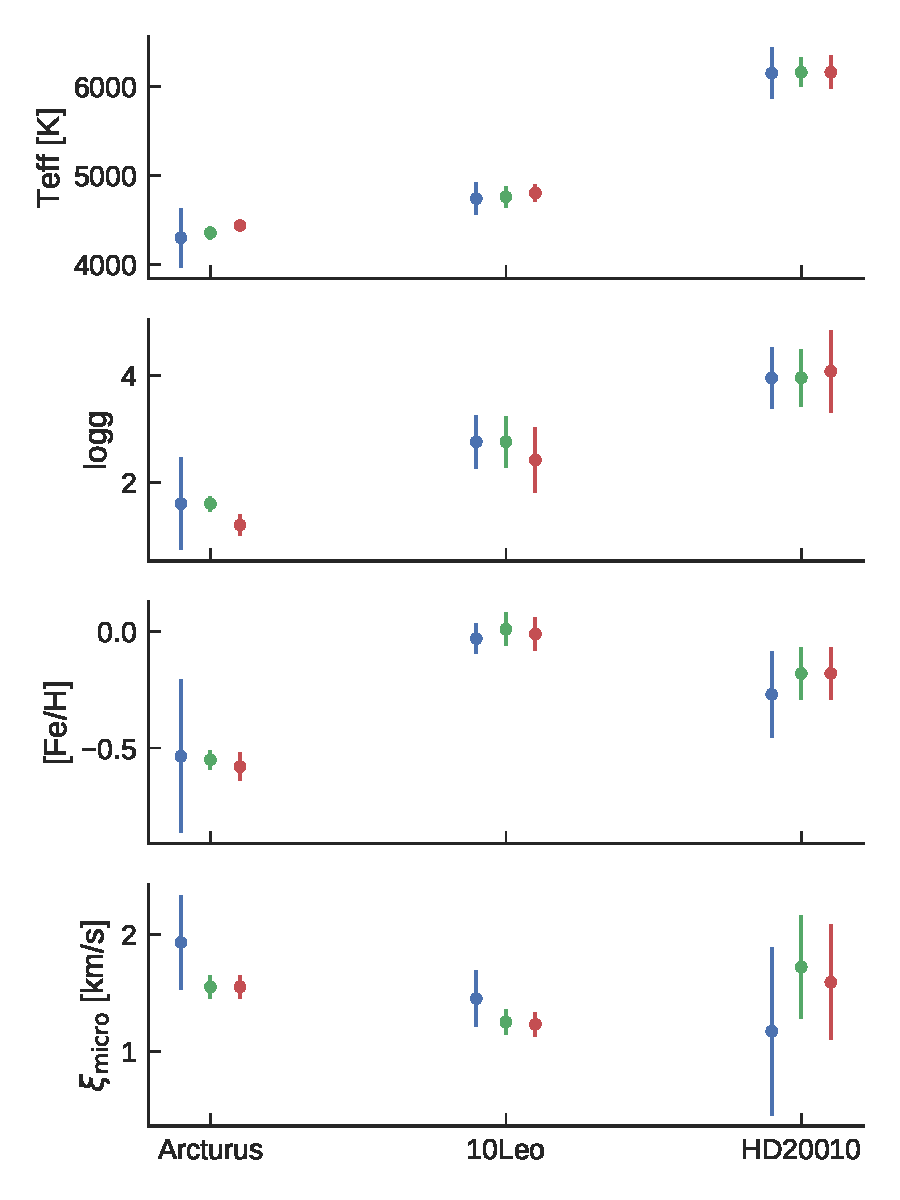
\includegraphics[width=1.0\linewidth]{figures/parameters.pdf}
    \caption{Parameters for Arcturus, 10 Leo, and HD 20010 (revisited in this
             paper). The blue points show the literature values from the PASTEL
             database as discussed in the text. The green points are the
             derived values with $\log g$ fixed to the literature value, and the
             red points show the derived parameters when $\log g$ is also
             derived.}
    \label{fig:parameters}
\end{figure}



\section{Arcturus}
\label{sec:arcturus}

Arcturus is one of the brightest stars on the night sky with a V magnitude of -0.05
\citep{Ducati2002}. Hence it is a prime target for testing with the numerous measurements of the
atmospheric parameters as mentioned above.

The atlas consists of both a summer observation set and a winter observation set. The two data sets
have been obtained in order to minimise the effect of tellurics at different spectral regions. A
comparison between the two sets of measured EWs - both the manual measurements using IRAF and the
automatic measurements using \ARES - are shown in Fig.~\ref{fig:EWcomp}. The automatic EW
measurements for the summer set and winter set show excellent agreement {\bf with a dispersion of
7m\AA{}}. This means that the two data sets are very similar, thus we decided to only manually
measure the EWs for one set (summer). We did, however, measure a few lines from the winter data set
to verify the agreement. {\bf Since the EWs are very similar we chose to only derive parameters of
the summer set with EWs measured with \ARES.} Parameters were derived with and without $\log g$ set
to a fixed value (1.60\,dex, the average literature value adopted). The derivation of the parameters
followed the procedure presented in Paper I, although we used the minimization routine of FASMA
\citep{Andreasen2017a}. After we reached convergence using all the iron lines we were able to
measure, one outlier above $3\sigma$ in abundance were removed, and the minimization routine was
restarted. This process was done iteratively until there were no more outliers. The final results
are presented in Table \ref{tab:results} together with mean parameters from the literature.

We generally see good agreement between the derived parameters and the average values from the
literature adopted (see Table \ref{tab:results}). The only parameter being difficult to measure is
the surface gravity due to the low number of \ion{Fe}{II} lines in the NIR. It is very important to
derive the metallicity accurately, and we report consistent results overall.


\section{10 Leo}
\label{sec:10Leo}

The approach for determining the atmospheric stellar parameters for 10 Leo is identical to Arcturus.
We use \ARES on each band (YJ, H, and K-band) separately. For the small gaps in the spectrum, we
simply set the flux to 1, since the spectrum is already normalised. This will also prevent \ARES to
identify and measure any lines in these regions. The EWs from the three regions are combined to one
final line list used for the determination of the parameters. {\bf The final results can be seen in
Fig.~\ref{fig:parameters} and Table~\ref{tab:results}.}

Generally the derived parameters are in excellent agreement with the literature values listed here.
{\bf For $T_\mathrm{eff}$ we were \SI{64}{K} off with $\log g$ set as a free parameter, well within
the errors. The only parameter that show a discrepancy compared to the literature value is
$\xi_\mathrm{micro}$ with a difference of \SI{0.22}{km/s}, which is at the limit of the errors
reported. We note that this parameter is not reported in the PASTEL database, and this was a derived
parameter from a empirical relation.} We were able to derive good $\log g$ values, although with
larger errors compared to the results from the literature.


\section{Synthetic cool stars}
\label{sec:synthetic_spectra}



\section{Parameter dependence on EP cut}
\label{sec:EPcut}

It is common practise, as in this case, to make a cut in EP for a line list when deriving
parameters. This was suggested in \citet{Andreasen2016} \citep[later done in][]{Andreasen2017b} for
the NIR line list used here. This cut was made at \SI{5.5}{eV}, inspired by a similar cut in the
optical \citep{Sousa2008a}, including only lines below this limit. The lines with higher EP might
also be affected by non-LTE effects which is not treated in this methodology.

As the parameters are dependent on this cut in EP\unfinished{Make a figure that shows this}, it
seemed interesting to divide a line list in two with upper and lower EPs and analyse those
separately. Before going into that analysis it is important to note, that the parameters should not
depend on any cut in EP if the theory is right, the radiative transfer code is working properly, and
the atmospheric models are correct. Lines with different EP are likely to be formed in different
layers of the atmosphere as discussed in \sref{sec:stellar_atmosphere}, however this should not
effect the final derived abundance, which is the problem here.
